\section{Behandling}
Behandlingsforløbet for et knæled med artrose har flere komponenter, behandlingen kan både kirurgiske og ikke-kirurgiske alt afhængt af graden af artrose.
\subsection*{Knæledet}
Knæet, \textit{articulatio genus}, er synovialt, sammensat led med en bevægelsesgrad fra 0 til 135$\degree$ fleksion til 0 til 5$\degree$ ekstension. Knæleddet er legemets største led, hvormed det også er udsat for større mekaniske påvirkninger end noget andet led i kroppen. Hermed er knæleddet hyppigere end noget andet led sæde for patologiske forandringer. Knæleddet er sammensat af 3 dele; \textit{femur}, \textit{tibia} og \textit{patella}. Disse er alle i slidfladerne beklædt med et tykt lag hyalinbrusk, op til 7 mm på femur. Sammen med meniskerne, der fordeler trykket på en større overflade, er hyalinbrusken med til at mindske friktionen i leddet. [Bevægeapperatets anatomi]

\begin{figure}[H] 
\begin{center}
\includegraphics[width=0.7\textwidth]{figures/bProblemanalyse/Artose_knae}
\end{center}
\caption{Når det normale knæ undergår patologiskeforandringer ved knæartrose vil strukturne i knæet forandre sig. Brusken kan ved infektion, slid eller traume blive beskadiget, hvilket vil eksponerer knoglen og førere til smerte.\citep{schroder} \citep{adobe}} 
\label{fig:tka_implant} 
\end{figure}

\subsection{Ikke-kiurgisk behandling}


%\subsection{Knæartrose}
%
%Knæartrose også kaldet slidgigt i knæene, har mange årsager. Hvor af nogle er overvægt, arv, traume eller tungt arbejde. Arterose er karakteriseret ved ødelæggelse af ledbrusken med dertil hørende reaktioner i de tillæggende knogler og slimhinder. Symptomerne på knæartrose er smerte, funktionstab og fejlstilling, hvilket besværliggøre hverdagen. 
%Ved knæartrose er sidste behandlings skridt kirurgi, afhængig af graden af traumet er forskellige kirurgiske indgreb en mulighed. [Nationale retningslinjer] 

\subsection{Kirurgisk behandling}

Når de ikke-kirurgiske behandlingsmuligheder har vise en utilstrækkelig effekt er kirurgi det næste skridt i behandlingsforløbet. Der findes flere behandlingsmuligheder inden for kirurgiskbehandling af artrose, hvor af der findes afarter af operationen afhængigt af den enkelte patients situation. Valget af operation og typen af den afhænger af flere faktorer, blandt andet patients alder, aktivitets niveau og hvor fremskreden artrosen er.

\subsubsection{Osteotomi}
Ved degenerative forandringer i knæleddet, grundet primær eller postttrumatisk knæledsarterose, kan patienter opleve belastningsreleaterede smerter, hvilket blandt andet kan skyldes fejlstilling. Osteotomi har tilfomål at afhjælpe den mekaniske belastning i det berørte område, for der ved at afhjælpe smerterne. Ved osteotomi fjernes en kile af knoglen(typisk tibia) og det resterende knogle sikres med skruer og metal plader, proceduren ændre knæets mekaniske akse, hvilket vil ændre belastningen af de degenererede områder.\citep{Osteotomi_og_TKA} Ved yngere(>50-65 år)\citep{Osteotomi_og_TKA} og aktive patienter vil der være større tilbøjlighed til at tilbyde osteotomi frem for den mere invasive TKA, derfor anbefales osteotomi af sundhedstyrelsen til behandling af mildere former for artrose med fejlstilling hos yngre og aktive patienter. [Nationale retningslinjer] Behandlingen ses som en temporær behandling der kan udskyde behovet for TKA, ifølge et Kohordestudie kan der forventes en smertelindring os 80\% af patienterne der får udført osteotomi. (79)(80) I følge [Nationale retningslinjer] må det forventes at 30-50\% af patienterne der får foretatget en osteotomi også vil få behov for en alloplastik operation. [Nationale retningslinjer] Tilbagevenden af smerter korreleres til tab af korrektionen, samt progression af artrosen. Hvorved en TKA kan komme på tale. \citep{Osteotomi_og_TKA} \textbf{Der er data på mere specifikke tilfredsheds undersøgelser, men ser ikke nogen trund til at medtage dem. }

\subsubsection{Alloplastik}
Alloplastik er et operativt indgreb der har til formål helt eller delvist at udskifte knæleddet, med specielt designede metal- og plastkomponenter som varig erstatning for bruskfladerne i knæet. Operationen opdeles i TKA og UKA, hvilket henholdsvis er helt eller delvis udskiftning af knæleddet og afhænger af den specifikke diagnose. Der kan ved traume tilfælde eller svære beskadigelser af de anatomiske strukturer omkring knæet forekomme specialiserede udgaver af knæalloplastik.

\begin{figure}[H] 
\begin{center}
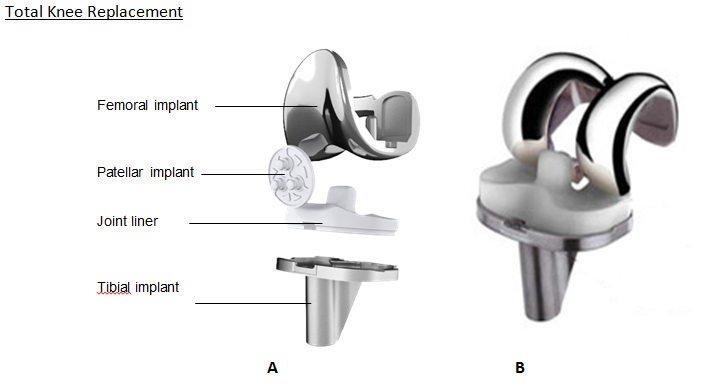
\includegraphics[width=0.7\textwidth]{figures/tka_implant}
\end{center}
\caption{Komponenterne til en total knæalloplastik, består af et femural og tibia implantat ofte bestående af en titaniumlegering. Patella- og tibiaindsatsen er lavet af polyethylen, hvilket er med til at mindske friktionen og efterligne knæledes naturlige bevægelse.\cite{1}} 
\label{fig:tka_implant} 
\end{figure}

Under selve operationen ligger patienten supineret på operationsbordet med knæet i en flekteret position. Et longitudinelt snit lægges over midten af patella. Patella og senerne eleveres og blotter knæleddet, hvilket giver kirurgen adgang til bruskfladerne på femur og tibia. Herefter fjerner kirurgen det ødelagte brusk, ved hjælp af en guideblok der skrues ind i femur og sikrer præcis fjernelse af den ønskede mængde væv. Dette gentages på tibia, hvorved der skabes plads til implantaterne. Midlertidige implantater indsættes for at sikre bevægelsesfriheden er bevaret og testes ved ekstension af knæet for at sikre at den rigtige mænge brusk og knogle materiale er fjernet. Når kirurgen er tilfreds med resultatet bores der guidehuller i henholdsvis femur, tibia og patella til fastemontering af de permanente implantater. Fastmontering sker ved at dække implantatet og monteringsstedet i bencement der limer proteserne fast til den eksisterende knogle struktur. Herefter sikres endnu engang at bevægelsesgraden er bibeholdt, førend indsnittet lukkes og operationen er fuldendt. En TKA operation varer typisk omkring én time, hvorefter patienten kan støtte på benet den følgende dag. Efter operationen følger et rehabiliteringsforløb for at støtte og styrke muskulaturen omkring knæet.\citep{Sanna2013} \citep{tka-technique}

I følge sundhedsstyrelsens vurdering er knæalloplastik, som behandling af knæartrose, effektiv til at mindske smerte, øge funktion og derved bedre livskvalitet.[Nationale retningslinjer] Holdbarheden af knæimplantaterne vurderes ud fra antallet af implantater der er blevet udskiftet efter 10 år, hvor det findes at 90 til 95\% af implantaterne ikke er revideret. Dog skal nævnes at det ikke er muligt at vurdere holdbarheden af den enkelte protese, da flertallet af patienter dør med en velfungerende implantat. [Nationale retningslinjer]

\paragraph{Succeskriterier}

Succeskriterier for behandlingen af arterose med kirurisk behandling kan ses fra et organisatorisk synspunkt samt et patient synspunkt. 

\textbf{Overgang til smerte afsnit.}
%
%(1) http://www.robodoc.com/patient_about_faqs.html
%
%(2) https://www.youtube.com/watch?v=tKji04oFGdU

% (3) http://www.ortopaedi.dk/fileadmin/Guidelines/Referenceprogrammer/Osteotomi_og_TKA.pdf

	%(4) Surgical approaches in total knee arthroplasty.
	
%	(5) tka-technique
%
%(79) Dahl AW, Toksvig-Larsen S, Roos EM. A 2-year prospective study of patient- relevant outcomes in patients operated on for knee osteoarthritis with tibial osteot- omy. BMC Musculoskeletal Disorders 2005;6(1):18. Er lagt på mendlay
%(80) Hoell S, Suttmoeller J, Stoll V, Fuchs S, Gosheger G. The high tibial osteoto- my, open versus closed wedge, a comparison of methods in 108 patients. Arch Or- thop Trauma Surg 2005;125(9):638-643. Er lagt på mendelay